
\documentclass[addpoints,12pt]{exam}
\usepackage{amssymb,amsmath,amsthm,graphicx}
\usepackage{tikz}
\usepackage{listings}
\usepackage{courier}
\usepackage{graphics}
\usepackage{scrextend}
\usepackage{adjustbox}

\lstset{frame=l,xleftmargin=\fboxsep,xrightmargin=-\fboxsep,colframe=gray}
\lstset{basicstyle=\ttfamily\footnotesize,breaklines=true}


\newcommand{\code}[1]{{\texttt{#1}}}
\newcommand{\mcode}[1]{{\text{\texttt{#1}}}}

\linespread{1.2}
\usepackage{color}
\definecolor{gray}{rgb}{0.3,0.3,0.3}



\pagestyle{headandfoot}
\runningheadrule
\firstpageheader{Math 9}{\,}{Practice Final}
\runningheader{Math 9}
              {\,}
              {Practice Final, Page \thepage\ of \numpages}
\firstpagefooter{}{}{}
\runningfooter{}{}{}
\newtheorem{theorem}{Theorem}
\newtheorem{definition}{Definition}
\newtheorem{expectation}{Expectation}

\newcommand{\RR}{\mathbb{R}}

\begin{document}
\begin{center}
\fbox{\fbox{\parbox{5.5in}{\centering
{\tt Directions:} The exam is 120 minutes long. Please read each question carefully. 
\vspace{10pt}

When asked to write code, you should write working Python code that has correct syntax. You should explain in 1-2 sentences what the idea for your solution is or write next to your code what it is doing. This will increase your chances of getting full/partial credit. 

Use the backs of the pages if needed.
}}}
\end{center}


\vspace{0.2in}

\makebox[\textwidth]{Last Name:\enspace\hrulefill}

\vspace{0.2in}

\makebox[\textwidth]{First Name:\enspace\hrulefill}

\vspace{0.2in}

\makebox[\textwidth]{Student ID \#:\enspace\hrulefill}

\vspace{0.2in}

\vspace{1in}

\gradetable

\newpage

\begin{questions}

\question[20]
Write down the output of the following programs.

\begin{enumerate}
\item 
\begin{lstlisting}[language=python]
x = 1
s = 0
for i in range(8):
    s += x
    x += 1
print(s)
\end{lstlisting}
\vfill
Answer: This computes $1+2+\dots+7 = 36$
\vfill


\item 
\begin{lstlisting}[language=python]
def f(n):
    if n > 0:
        return n * g(n)
    return 1

def g(n):
    return f(n // 2)

print(f(6))
\end{lstlisting}
\vfill
Answer: $f(6) = 6 * g(6)$, $g(6) = f(3)$, $f(3) = 3 * g(3)$, $g(3) = f(1)$, $f(1) = 1*g(1)$, $g(1) = f(0)$, $f(0) = 1$. So $f(6) = 6*3*1 = 18$
\vfill

\item 
\begin{lstlisting}[language=python]
from functools import reduce
x = reduce(lambda a,d: 2*a+d, [1,0,0,0,0,1,0,1])
print(x)
\end{lstlisting}
\vfill
Answer: Recall how the reduce function works. You apply the function to the first two elements, then apply the function to the answer and the next element,\dots In this case you keep multiplying by two and adding. The answer is 133. 
If you think about it, you will notice that this computes the base 10 version of the binary number.
\vfill

\item 
\begin{lstlisting}[language=python]
def f(xs):
    if xs == []:
        return 0
    return xs[0] + f(xs[1:])

f([1,2,3,4,5])
\end{lstlisting}
\vfill
Answer: \code{f([1,2,3,4,5] = 1 + f([2,3,4,5]))}, 
\\\code{f(2,3,4,5) = 2 + f([3,4,5])},\dots
It's computing the sum. Which is 15.
\vfill


\end{enumerate}

\newpage
\question[20] Produce the following lists without using for or while loops. 
\begin{enumerate}
  \item \code{[0, 1, 3, 7, 15, 31, 63, 127, 255, 511]}
    
    \vspace{0.3in}
    Solution: Powers of two minus 1. 
    
    \code{[2 ** x - 1 for x in range(10)]}
    \vfill
  \item \code{[1, 2, 4, 5, 7, 8, 10, 11, 13, 14, 16, 17, 19]}

    \vspace{0.3in}
    Solution: all the numbers except multiples of 3. 
    
    \code{[x for x in range(20) if x \% 3 != 0]}
    \vfill
  \item \code{[-1, 2, -3, 4, -5, 6, -7, 8, -9, 10, -11, 12, -13, 14]}
    
    \vspace{0.3in}
    Solution: all the numbers in range but multiply by alternating sign. 
    
    \code{[x * (-1)**x for x in range(1,15)]}
    \vfill
\end{enumerate}


\newpage
\question[20] Write code that will produce the following graphs (or something that looks like it; use \code{plt.plot(X, Y)} and \code{plt.scatter(X, Y)}).
\begin{enumerate}
\item
\adjustbox{valign=t}{
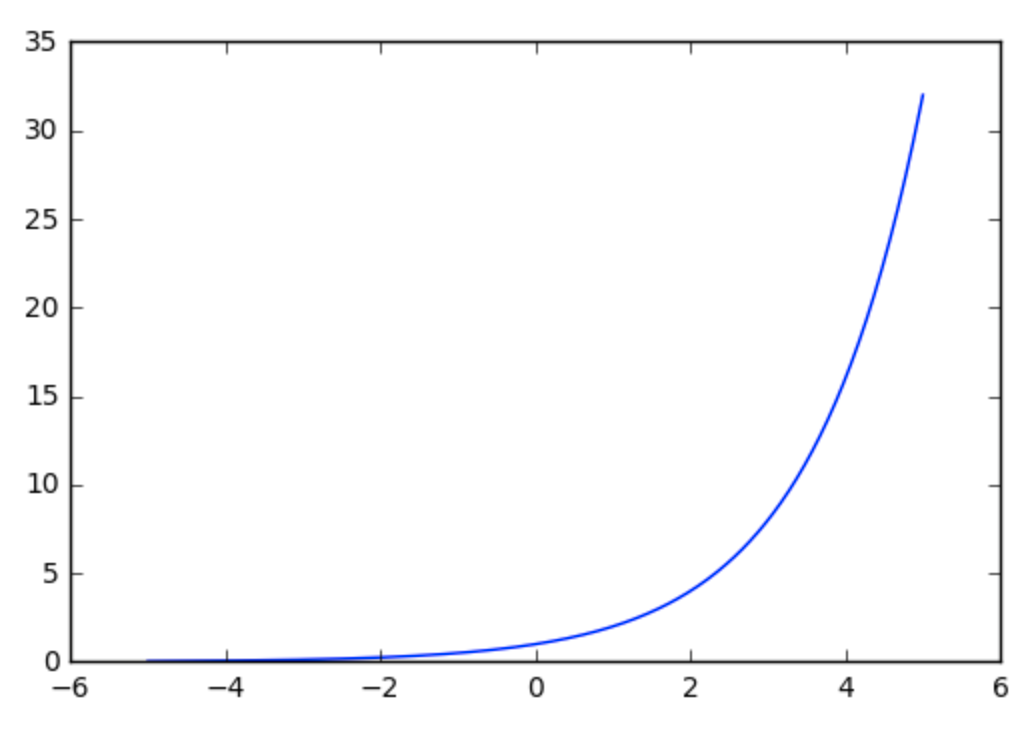
\includegraphics[valign=t, width=3.1in]{graph_exp.png}
}
\vspace{0.2in}

Solution: exponential function. 
\begin{lstlisting}[language=python]
X = np.linspace(-5,5,400)
Y = 2 ** X
plt.plot(X, Y)
\end{lstlisting}
(it doesn't matter if you said \code{2**x} or some other exponential)
\vfill
\item 
\adjustbox{valign=t}{
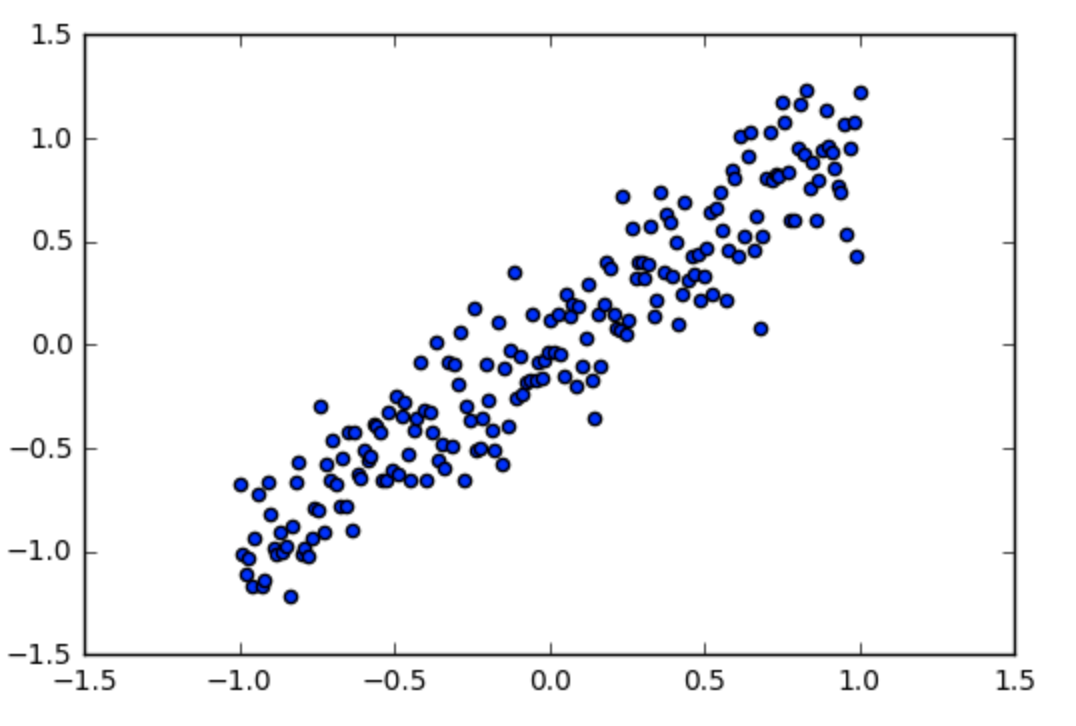
\includegraphics[valign=t, width=3.2in]{graph_noise_lin.png}
}

\vspace{0.2in}

Solution: adding some noise to $y=x$.
\begin{lstlisting}[language=python]
X = np.linspace(-1,1,200)
Y = X + np.random.normal(0,0.2,X.shape[0])
plt.scatter(X, Y)
\end{lstlisting}
(Of course, the 0.2 doesn't matter as long as you knew how to add some noise.)


\vfill
\end{enumerate}


\newpage
\question[20] Complete the code below to implement the function \code{chessboard(n)} that will return a numpy array with 1's and 0's arranged in a chessboard pattern. You can assume \code{n} is odd. 
Examples:
\begin{lstlisting}[language=python]
In:   chessboard(3)
Out:  array([[0, 1, 0],
             [1, 0, 1],
             [0, 1, 0]])

In:   chessboard(5)
Out   array([[0, 1, 0, 1, 0],
             [1, 0, 1, 0, 1],
             [0, 1, 0, 1, 0],
             [1, 0, 1, 0, 1],
             [0, 1, 0, 1, 0]])
\end{lstlisting}

\vspace{0.2in}
Solution: reshape an array with alternating 0's and 1's. 
\begin{lstlisting}[language=python]
def chessboard(n):
    X = np.array([x % 2 for x in range(n * n)]).reshape([n,n])
    return X
\end{lstlisting}
\vfill

Complete the code below to implement the function \code{chessgonewrong(n)}, which produces a chess-board with the middle $3\times 3$ square having $-1$'s instead of $1$s.
\begin{lstlisting}[language=python]
In:   chessgonewrong(7) 
Out:  array([[ 0,  1,  0,  1,  0,  1,  0],
             [ 1,  0,  1,  0,  1,  0,  1],
             [ 0,  1,  0, -1,  0,  1,  0],
             [ 1,  0, -1,  0, -1,  0,  1],
             [ 0,  1,  0, -1,  0,  1,  0],
             [ 1,  0,  1,  0,  1,  0,  1],
             [ 0,  1,  0,  1,  0,  1,  0]])
\end{lstlisting}

\begin{lstlisting}[language=python]
def chessgonewrong(n):
    X = chessboard(n)

    return X
\end{lstlisting}

\vspace{0.2in}
Solution: multiply a $3\times3$ square at the center by -1.
\begin{lstlisting}[language=python]
def chessgonewrong(n):
    X = chessboard(n)
    X[n // 2 - 1 : n // 2 + 2, n // 2 - 1 : n // 2 + 2] *= -1
    return X
\end{lstlisting}
\vfill


\vfill


\newpage
\question[20] Implement a function \code{divisors(n)} that returns all positive integer divisors of an integer \code{n} as a list. (returns not prints)


\vspace{0.8in}

Solution: Loop through i=1,\dots,n and add them to the list if they divide. 
\begin{lstlisting}[language=python]
def divisors(n):
    xs = []
    for i in range(1,n+1):
        if n % i == 0:
            xs.append(i)
    return xs
\end{lstlisting}


\newpage
\question[20] A palindrome is a word that is the same when reversed, e.g. ``amanaplanacanalpanama''. Write a function \code{ispalin(s)} that will return \code{True} if a string \code{s} is a palindrome and \code{False} otherwise. (remark: you can work with \code{s} as if it were a list). 

\vspace{0.8in}
Solution: as you loop to the middle, check to see if the character matches with the corresponding character from the other side. If there are any mismatches, return False. If you finish the loop without any mismatches, then return True. 
\vspace{0.2in}

\begin{lstlisting}[language=python]
def ispalin(s):
    n = len(s)
    for i in range(n//2):
        if s[i] != s[n-1-i]:
            return False
    return True
\end{lstlisting}

\newpage
\question[20] Recall the \code{Polynomial} class from the homework that stores a polynomial as a list of its coefficients. Implement the \code{\_\_add\_\_(self, other)} function that returns a new polynomial which represents the sum of the polynomials \code{self} and \code{other}.  

\begin{lstlisting}[language=python]
class Polynomial():
    def __init__(self, xs):
        self.coeffs = xs
   
    # returns a string representation of the polynomial
    def __repr__(self):
        if self.coeffs == []:
            return "0"
        c = ""
        for i, x in enumerate(self.coeffs):
            c += str(x) + "x" + "^" + str(i) + " + "
        return c[:-3]
    
    def __add__(self, other):
\end{lstlisting}


\vspace{0.8in}
Solution: This was a problem in Homework 5. You add the corresponding coefficients (but have to be careful about not getting index out of bounds errors because you are looking too far to the right).

\begin{lstlisting}[language=python]
    def __add__(self, other):
        i = 0
        new_coeffs = [0.0 for i in range(max(len(self.coeffs), len(other.coeffs)))]
        for i in range(len(new_coeffs)):
            coefa = self.coeffs[i] if i < len(self.coeffs) else 0.0
            coefb = other.coeffs[i] if i < len(other.coeffs) else 0.0
            new_coeffs[i] = coefa + coefb
        return Polynomial(new_coeffs)

\end{lstlisting}

\newpage
\question[20] Write code that will find the minimum of the function $f(x,y) = x^4 + y^2 + 2x + 4y + 1$ using gradient descent. (Start the descent from $(x,y) = (5,5)$ and use the learning rate of $\eta = 0.01$). Your code should print the minimum value it finds. 


\vspace{0.8in}
Solution: Please refer to the lecture notes on gradient descent for a careful explanation. 

\vspace{0.2in}
\begin{lstlisting}[language=python]
f = lambda x, y: x**4 + y**2 + 2*x + 4*y + 1
delfdelx = lambda x, y: 4 * x**3 + 2
delfdely = lambda x, y: 2*y + 4

num_steps = 1000
eta = 0.01
x = 5
y = 5
for i in range(num_steps):
    dx = delfdelx(x,y)
    dy = delfdely(x,y)
    x -= eta * dx
    y -= eta * dy

print(x,y,f(x,y))
\end{lstlisting}

\end{questions}
\end{document}
